\chapter{Instalación}
    \section{Armado} 
        Este prototipo cuenta con un panel solar como medio de obtención de energía renovable, pero podría utilizarse cualquier otro tipo de generador de energía.\par
        Para evitar atenciones agravadas por la distancia recorrida a través de los cables de conexión, recomendamos colocar la batería cerca del panel solar, u otros, preferentemente en un ambiente cerrado o protegido de la intemperie.\par
        Luego de elegir un espacio protegido de la humedad u otros factores climáticos, alejado de zonas de tránsito recurrente, o habituadas por niños y animales, quitar el embalaje de todas las piezas y prepararlas para su posterior uso.\par
        Recomendamos observar continuamente la foto del dispositivo armado para chequear la posición de cada pieza.\par
        Al ajustar cada bulón, hace falta utilizar una llave de 17mm, y una llave álem de 6mm por el otro lado.\par
        Recomendamos contar con un juego de llaves criquet para facilitar el proceso. Ambas llaves colocadas en simultáneo, con la rosca preparada para un ajuste.\par
        Tener en cuenta, que luego de algunos armados y desarmados las roscas de los bulones y las tuercas pueden verse deterioradas, es importante observar particularmente este punto antes de cada instalación, y reemplazar las piezas en caso de ser necesario. Recomendamos reemplazar en su totalidad los 12 pares de bulón-tuerca cuando uno de ellos aparezca deteriorado.\par
        A continuación, los pasos a seguir:\par

        \begin{enumerate}
            \item Colocar la estructura inferior sobre el suelo.
            \item Tomar uno de los caños de 230cm, y posicionarlo en su lugar.
            \item Ajustar el bulón y la tuerca correspondiente a dicha unión.
            \item Tomar una vara de 87cm de largo, presentarla a modo de escuadra o soporte entre la estructura inferior y el caño vertical, colocado del lado externo a la estructura.
            \item Tomar el caño de 230cm restante y repetir los pasos 2, 3 y 4.
            \item Colocar los dos soportes o escuadras restantes, ajustando únicamente la parte inferior, la pieza quedará haciendo péndulo sobre el caño vertical.
            \item El paso que sigue es posicionar la estructura superior, para esto será necesaria la ayuda de otra persona, esta se quedará sosteniendo la estructura desde el frente, mientras la otra persona ajusta ambos lados de la pieza.
            \item Luego habrá que terminar de colocar los dos soportes colocados en el paso 6, la persona que se encuentra sosteniendo la estructura no podrá soltarla hasta que uno de los dos soportes esté ajustado totalmente.
        \end{enumerate}
        
        La estructura se encuentra armada, ahora hay que colocar el peso y la carga:\par

        \begin{enumerate}
            \item Presentar el motor del dispositivo sobre su respectivo soporte. Ajustar parcialmente la abrazadera a su alrededor.
            \item Tomar las dos varillas roscadas de 5 cm con sus respectivas tuercas y arandelas, ajustando ambas para que mantengan el motor en posición.
            \item Una vez ajustados los soportes, terminar de ajustar la abrazadera, el motor debe estar fijo en su posición.
            \item Tomar el encoder y asegurarlo a la polea adherida al motor. Dejar a disposición sus terminales para su posterior conexión.
            \item Colocar sobre el suelo, debajo de la estructura el banco de soporte previamente seleccionado para sostener el peso.
            \item Trasladar con ayuda de otra persona el mismo hasta posicionarlo sobre dicho banco. Es importante observar que el cable se encuentre adherido al peso por la parte inferior del mismo.
            \item Colocar el cable en los rieles de las 4 poleas.
            \item Asegurando que el ojo de gancho esté lo más abierto posible, colocar el acople 1 entre el peso y la punta del ojo de gancho que no está adherida al cable.
            \item Una vez colocado, cerrar el ojo de gancho lo máximo posible, asegurándose de no girar sobre sí mismo el cable. Recomendamos el uso de una varilla a modo de palanca.
        \end{enumerate}
        
        El dispositivo está armado, resta conectar el panel solar al sistema, el encoder y los terminales del motor.\par
        Asegurarse de que el panel solar se encuentre posicionado y con sus dos terminales disponibles para su conexión. Es importante que en ningún momento se toquen los terminales para evitar dañar el dispositivo.\par
        
        Finalmente:\par

        \begin{enumerate}
            \item Conectar los terminales del encoder a sus respectivas borneras, teniendo en cuenta:

            \begin{itemize} [label=-]
                \item Pin A: Verde
                \item Pin B: Blanco
                \item VCC: Rojo
                \item GND: Negro
                \item Malla de recubrimiento: Malla metálica
            \end{itemize}

            \begin{figure} [H]
                \centering
                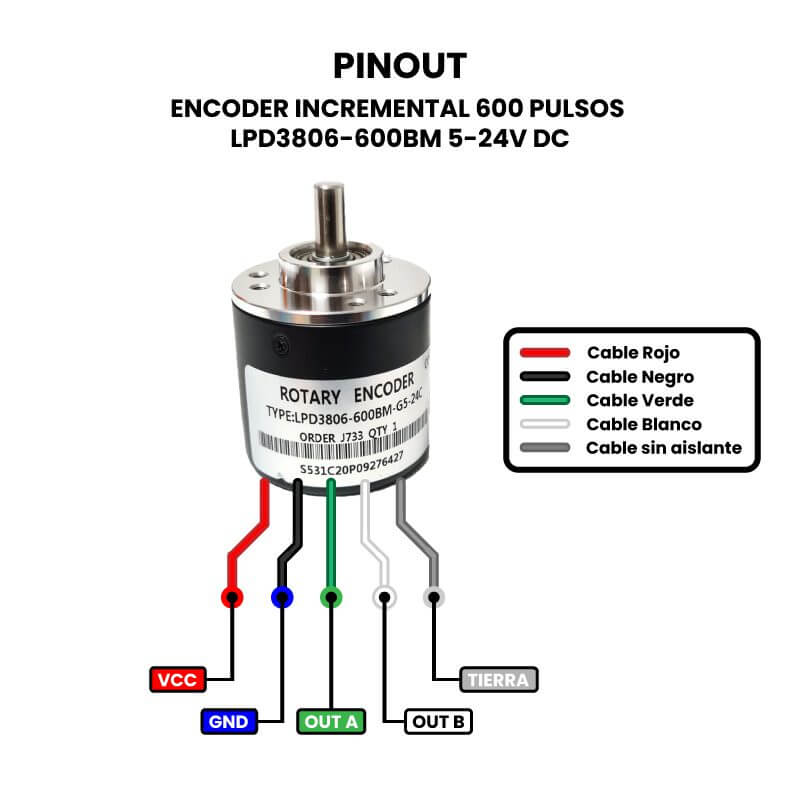
\includegraphics[width=0.5\linewidth]{Imagenes/Instalacion/Encoder.png}
            \end{figure}
            
            \item Conectar los terminales del motor a sus respectivas borneras.
            \item Conectar los terminales del panel solar a sus respectivas borneras.

        \end{enumerate}

        \begin{figure}
            \centering
            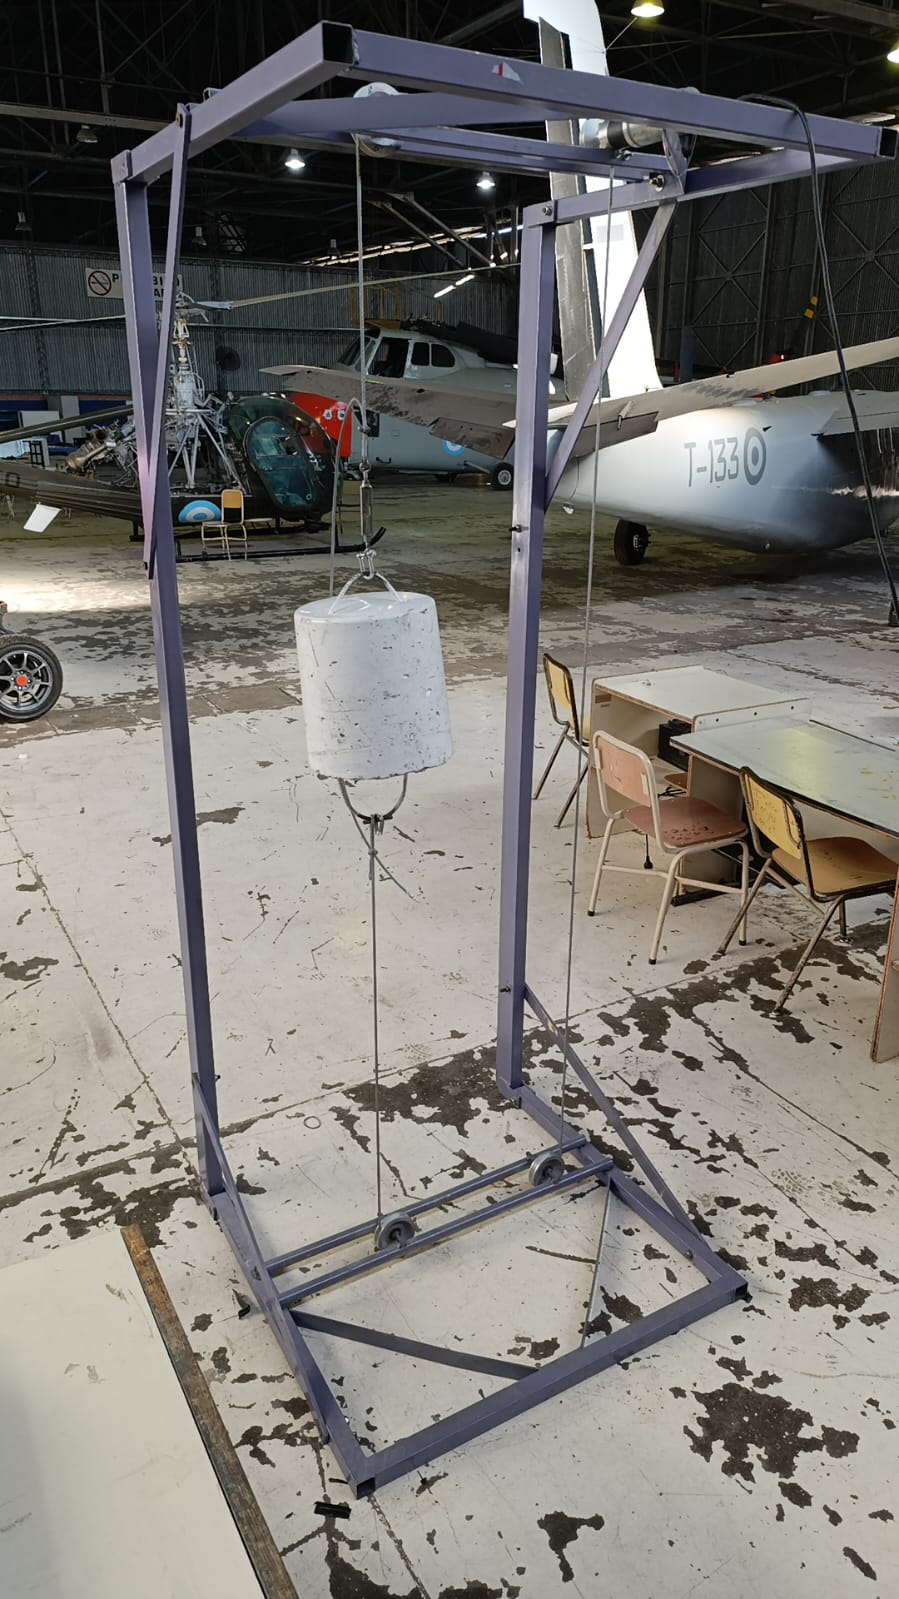
\includegraphics[width=0.5\linewidth]{Imagenes/Instalacion/Estructura.png}
        \end{figure}